% !TEX root =../main.tex

\chapter{Beispiel}

Hier etwas Text zur Einleitung. Ye ist meine absolute Lieblings Ye.

\section{Ziel der Arbeit}

Ja, wir finden auch, dass man über die Copy noch mal reden sollte. Das hier kann es jedenfalls nicht sein. Das klingt ja wie auf dem Totenbett getextet. Da muss wesentlich mehr Produktaussage rein. Ja, wir finden auch, dass man über die Copy noch mal reden sollte. Das hier kann es jedenfalls nicht sein. Das klingt ja wie auf dem Totenbett getextet. Da muss wesentlich mehr Produktaussage rein. Ja, wir finden auch, dass man über die Copy noch mal reden sollte.

\subsection{Motivation}

Ja, wir finden auch, dass man über die Copy noch mal reden sollte. Das hier kann es jedenfalls nicht sein. Das klingt ja wie auf dem Totenbett getextet. Da muss wesentlich mehr Produktaussage rein. Ja, wir finden auch, dass man über die Copy noch mal reden sollte. Das hier kann es jedenfalls nicht sein. Das klingt ja wie auf dem Totenbett getextet. Da muss wesentlich mehr Produktaussage rein. Ja, wir finden auch, dass man über die Copy noch mal reden sollte.

\subsubsection{Meine Motivation}

Ja, wir finden auch, dass man über die Copy noch mal reden sollte. Das hier kann es jedenfalls nicht sein. Das klingt ja wie auf dem Totenbett getextet. Da muss wesentlich mehr Produktaussage rein. Ja, wir finden auch, dass man über die Copy noch mal reden sollte. Das hier kann es jedenfalls nicht sein. Das klingt ja wie auf dem Totenbett getextet. Da muss wesentlich mehr Produktaussage rein. Ja, wir finden auch, dass man über die Copy noch mal reden sollte.

\paragraph{Ein Paragraph}

Ja, wir finden auch, dass man über die Copy noch mal reden sollte. Das hier kann es jedenfalls nicht sein. Das klingt ja wie auf dem Totenbett getextet. Da muss wesentlich mehr Produktaussage rein. Ja, wir finden auch, dass man über die Copy noch mal reden sollte. Das hier kann es jedenfalls nicht sein. Das klingt ja wie auf dem Totenbett getextet. Da muss wesentlich mehr Produktaussage rein. Ja, wir finden auch, dass man über die Copy noch mal reden sollte.

\subparagraph{Ein Unterparagraph}

Ja, wir finden auch, dass man über die Copy noch mal reden sollte. Das hier kann es jedenfalls nicht sein. Das klingt ja wie auf dem Totenbett getextet. Da muss wesentlich mehr Produktaussage rein. Ja, wir finden auch, dass man über die Copy noch mal reden sollte. Das hier kann es jedenfalls nicht sein. Das klingt ja wie auf dem Totenbett getextet. Da muss wesentlich mehr Produktaussage rein. Ja, wir finden auch, dass man über die Copy noch mal reden sollte.

\section{Textformatierung}

\section{Abbildungen}

In der Abbildung \vref{fig:wursthund} ist der so genannte Wursthund in seiner natürlichen Umgebung zu sehen.

\begin{figure}[htbp]
	\centering
	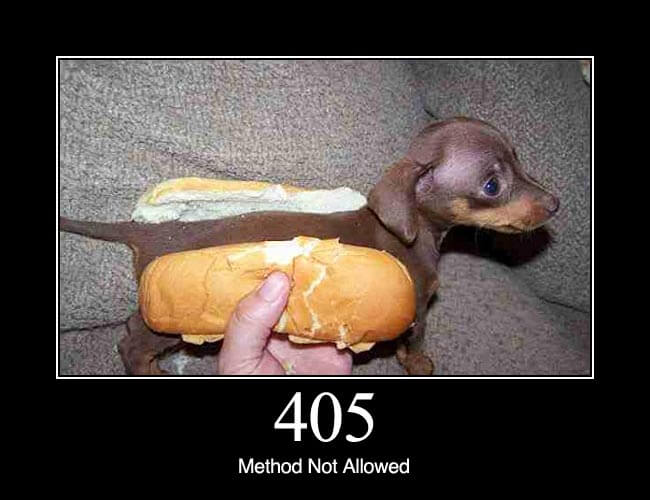
\includegraphics[width=10cm]{bilder/wursthund.jpg}
	\caption{Wursthund}
	\label{fig:wursthund}
\end{figure}

\section{Tabellen}

Eine kleine Tabelle, welche nicht durch Seitenumbrüche aufgetrennt werden kann, ist in Tabelle \ref{tab:kleine-tabelle} zu sehen.

\begin{table}[htbp]
\centering
\begin{tabular}{lcr}
                   & Zeiten       & \\
Ziel            & Abfahrt    & Dauer \\
Frankfurt & stündlich & 3:20 \\
Berlin        & stündlich & 5:40 \\
Hamburg & alle 5\,h   & 5:20 \\
\end{tabular}
\caption{Tabelle mit variabler Spaltenbreite}
\end{table}

\begin{table}[htbp]
\centering
\begin{tabular}{| p{3.5cm} | p{10.5cm} |}
\hline
\textbf{Spalte 1}& \textbf{Spalte 2}\\
\hline
\textbf{Eintrag 1}& \textbf{Eintrag 2}\\
Daten& Daten\\
Daten& Daten\\
Daten& Daten\\
\hline
\textbf{Eintrag 1}& \textbf{Eintrag 2}\\
Daten& Daten\\
Daten& Daten\\
Daten& Daten\\
\hline
\end{tabular}
\caption{Kleine Tabelle}
\label{tab:kleine-tabelle}
\end{table}

Eine lange Tabelle, welche sich über mehrere Seiten erstrecken kann ist in Tabelle \ref{tab:lange-tabelle} dargestellt.

\begin{longtable}{|p{2cm} | p{2cm} | p{2cm} | p{2cm} | p{2cm} |}
\hline
\textbf{\O min}& \textbf{\O max}& \textbf{Wert 1}& \textbf{Wert 2}& \textbf{Wert 3}\\
\hline
6& 10& 56& 100& 20,00\\
\hline
6& 10& 100& 150& 20,00\\
\hline
6& 10& 150& 200& 20,00\\
\hline
6& 10& 200& 250& 20,00\\
\hline
6& 10& 250& 300& 20,00\\
\hline
6& 10& 300& 350& 20,00\\
\hline
6& 10& 350& 400& 20,00\\
\hline
10& 14& 63& 100& 20,00\\
\hline
10& 14& 100& 150& 20,00\\
\hline
10& 14& 150& 200& 20,00\\
\hline
10& 14& 200& 250& 20,00\\
\hline
10& 14& 250& 300& 20,00\\
\hline
10& 14& 300& 350& 20,00\\
\hline
10& 14& 350& 400& 20,00\\
\hline
\caption{Lange Tabelle}
\label{tab:lange-tabelle}
\end{longtable}

\section{Verweise}

Es existieren mehrere Arten auf Objekte zu verweisen.

Abbildungsnummer: \ref{fig:wursthund}

Abbildungsnummer und relative Seitenzahl: \vref{fig:wursthund}

Seitenzahl: \pageref{fig:wursthund}

Relative Seitenzahl: \vpageref{fig:wursthund}

\section{Beschreibungsumgebung}

\section{Quellenangabe}